\subsection{Wellendiskussion}
\label{sec:wellen:diskussionwellenform}
W"ahrend wir anschliessend mit der Rekursionsformel L"osungen der 
Differentialgleichung (\ref{eq:wellen:pxdgl}) mit parabolischen Profil
geplottet haben, entdeckten wir, dass die L"osung $y(x)$ ihre Form 
bei den jeweiligen Nullstellen des Profils $p(x)$ wechselt.
Vergleichen wir die Wellenformen der Abbildungen \ref{fig:wellen:variablec} und 
\ref{fig:wellen:variablea} mit den Abbildungen \ref{fig:wellen:sin-cos} und 
\ref{fig:wellen:sinh-cosh}, stellt sich heraus, dass die L"osung der 
Titelgleichung eng mit der gefundenen L"osung der Gleichung 
(\ref{eq:wellen:lineareDGL}) verwandt ist. So k"onnen die L"osungen des 
parabolischen Profils als verschiedene $c$ Werte der linearen 
Differentialgleichung verstanden werden, welche in die L"osungsgleichung 
(\ref{eq:wellen:loesunglineareDGL}) eingesetzt werden k"onnen. 
Da mit einem $c$, respektive mit einer L"osung des Profils nur ein Punkt 
und nicht die ganze Funktion beschrieben wird, lassen sich die Konstanten $C_1$ 
und $C_2$ aus der Gleichung (\ref{eq:wellen:loesunglineareDGL}) nicht mehr 
allgemein bestimmen. Es gibt ausserdem keine reinen trigonometrischen Formen 
mehr, sondern geht die Welle f"ur negative Profill"osungen in die 
hyperbolischen Funktionen Sinus Hyperbolicus und Cosinus Hyperbolicus und f"ur 
positive in Sinus und Cosinus über.

Die Wellenformen sind bei variablem $c$ (Abbildung \ref{fig:wellen:variablec}) 
und $a$ (Abbildung \ref{fig:wellen:variablea}) alle "ahnlich, da sich ausser 
den Nullstellen und dem $y$-Achsen Schnittpunkt der Profilgleichung $p(x)$ 
nichts ver"andert. Unterschiedliche $a$-Werte f"uhren haupts"achlich zu einer 
ver"anderten Frequenz der Welle. Zwar hat dieser Parameter auch Auswirkungen 
auf die Amplitude, jedoch wird diese mehrheitlich durch den $c$-Wert 
beeinflusst, welcher daf"ur nur einen kleinen Einfluss auf die Frequenz hat.

\begin{figure}
	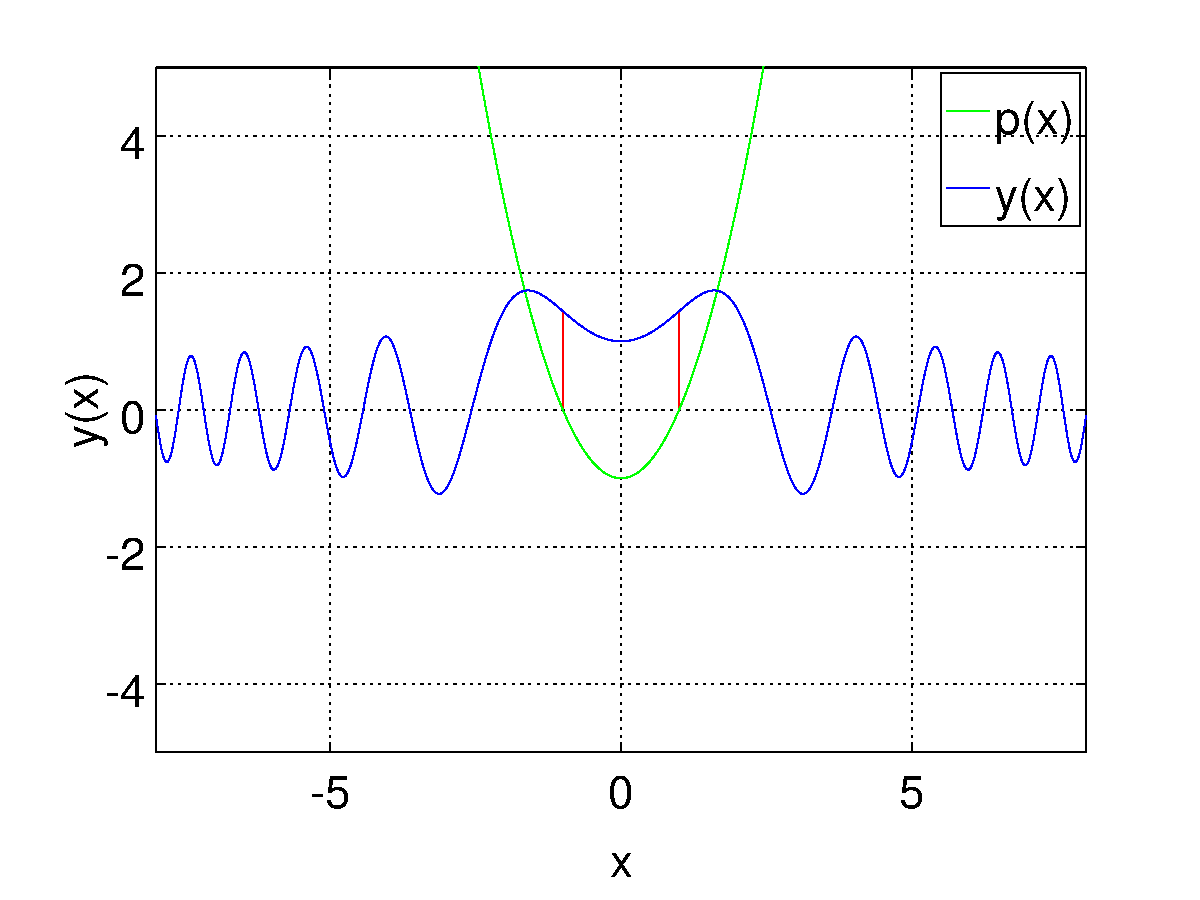
\includegraphics[width=0.5\hsize]{./wellen/images/varc/varc1.pdf}
	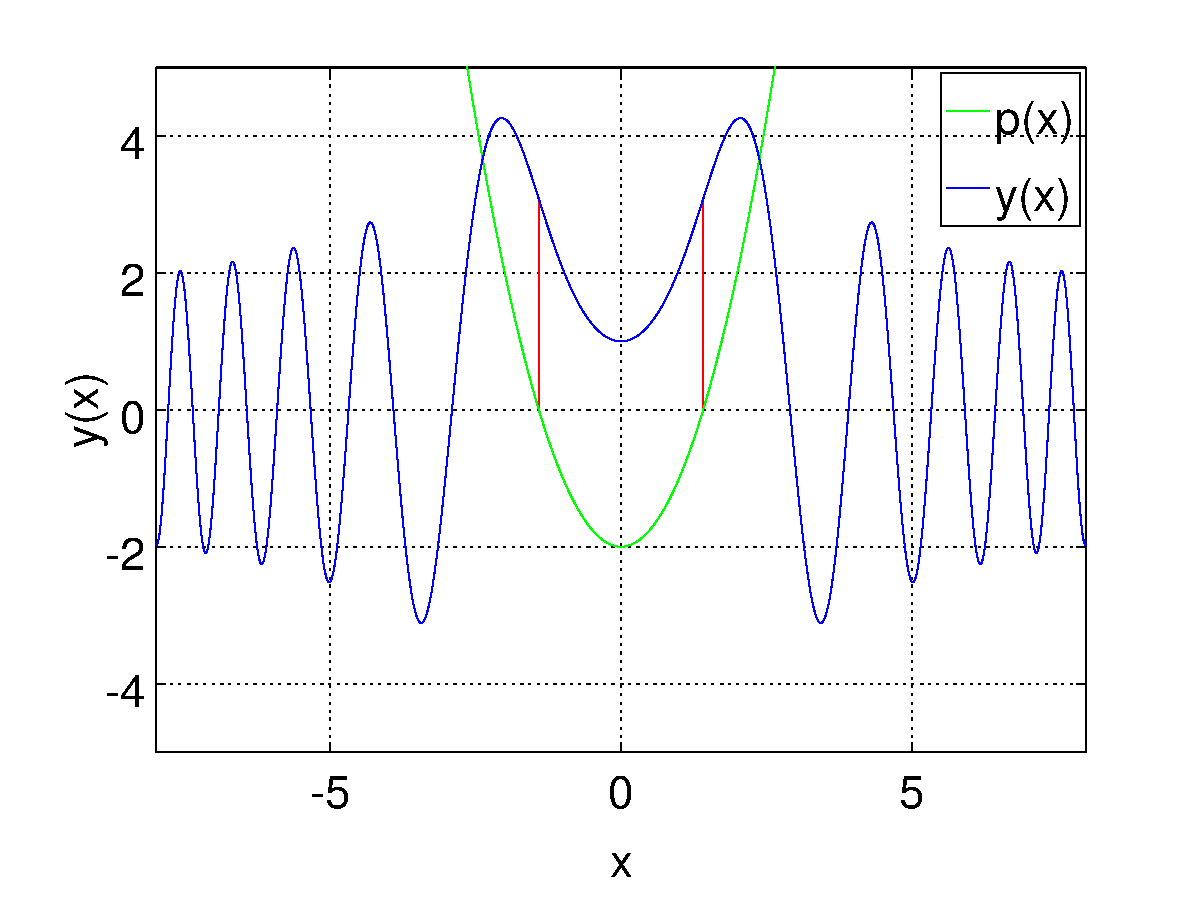
\includegraphics[width=0.5\hsize]{./wellen/images/varc/varc2.pdf}
	\caption{Wellenform mit unterschiedlichen $c$ Werten (links $c = -1$, 
	rechts $c = -2$).}
	\label{fig:wellen:variablec}
\end{figure}

\begin{figure}
	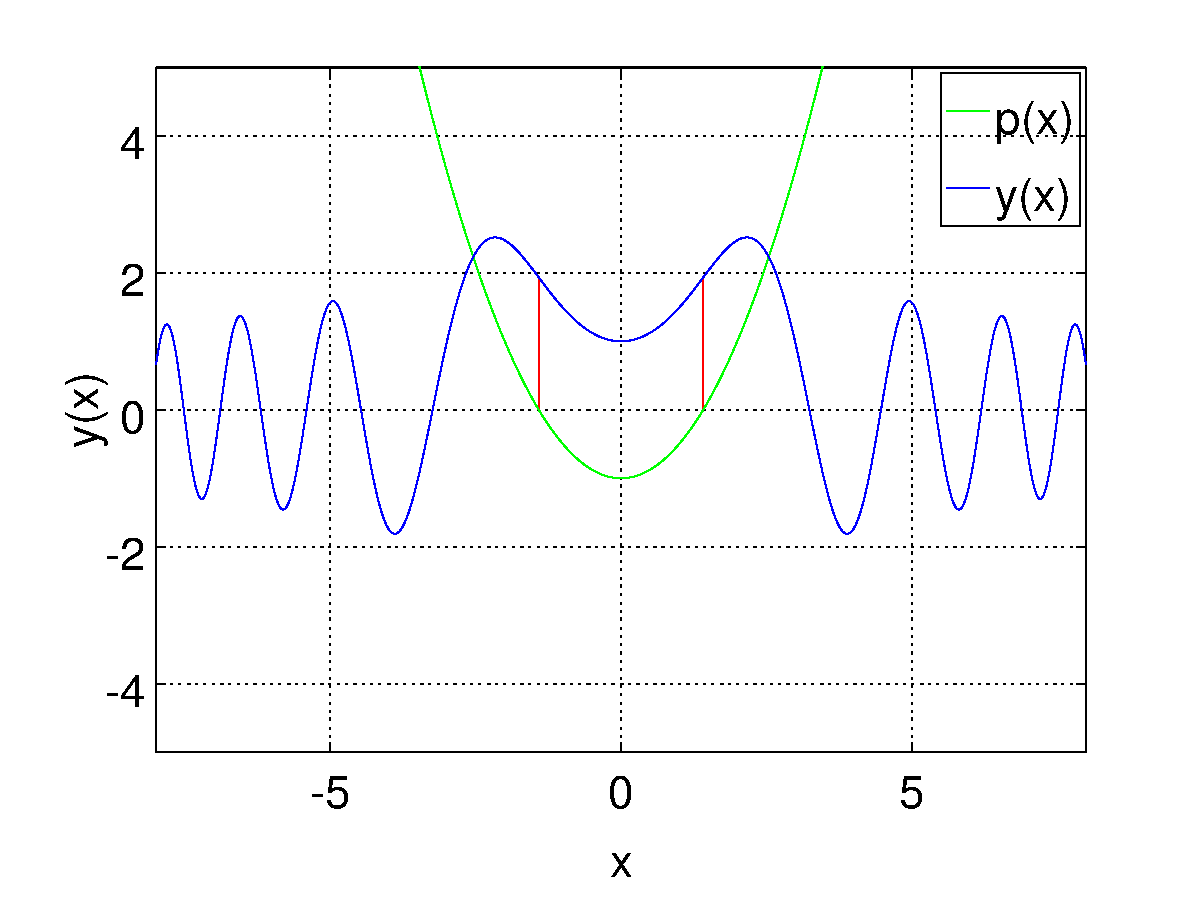
\includegraphics[width=0.5\hsize]{./wellen/images/vara/vara1.pdf}
	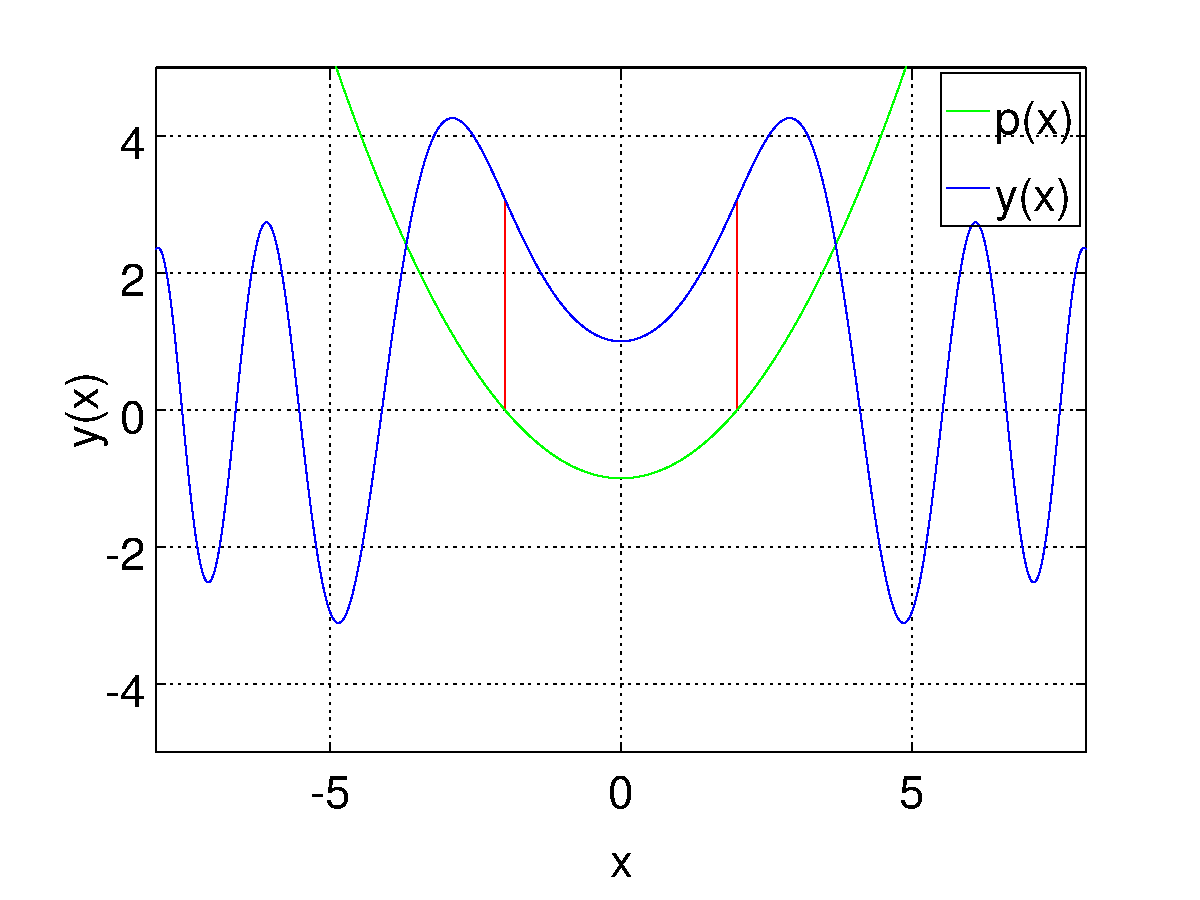
\includegraphics[width=0.5\hsize]{./wellen/images/vara/vara2.pdf}
	\caption{Wellenform bei unterschiedlichen $a$ Werten (links $a = 0.5$, 
	rechts $a = 0.25$).}
	\label{fig:wellen:variablea}
\end{figure}

Mit dieser Diskussion verlassen wir das parabolische Profil und betrachten 
allgemeinere Aspekte wie Stolpersteine bei der Ausf"uhrung solcher Berechnungen 
oder die verallgemeinerte L"osung von Differentialgleichungen 
dieser Art mit einem Profil der Form
\begin{equation*}
p(x) = \sum_{i=0}^{n} \lambda_i x^i.
\end{equation*}
